\documentclass{article}
\usepackage[utf8]{inputenc}
\usepackage{geometry}
\usepackage{pdfpages}
\usepackage{mathtools}
\usepackage{array}
\usepackage{filecontents}
\usepackage{nicematrix}
\usepackage{bodeplot}
\graphicspath{{images/}}
\geometry{
	a4paper,
	total={170mm,257mm},
	left=20mm,
	top=20mm,
}
\usepackage{graphicx}
\usepackage{titling}
\usepackage[american,RPvoltages]{circuiTikz}
\usepackage{tikz, tikz-cd}
\usepackage{pgfplots}
\usepackage{siunitx}
\usepackage{float}
\usepackage{enumitem}
\usepackage{amsmath,amsfonts,stmaryrd,amssymb} % Math packages
\usepackage{schemabloc}
\usepackage{tcolorbox}
\usepackage{xcolor}
\usetikzlibrary{positioning}
\usepackage[scr]{rsfso}
%\usepackage{tgpagella} 

\newcommand*{\Scale}[2][4]{\scalebox{#1}{$#2$}}%
\newcommand*{\Resize}[2]{\resizebox{#1}{!}{$#2$}}%

\newcommand{\Laplace}{\mathscr{L}}

\title{Relación del tiempo de subida a constante de tiempo}
\author{Rodrigo Castillejos}
\date{Agosto 2024}

\usepackage{fancyhdr}
\fancypagestyle{plain}{%  the preset of fancyhdr 
	\fancyhf{} % clear all header and footer fields
	\fancyfoot[L]{\thedate}
	\fancyhead[L]{Análisis de circuito con OpAmp}
	\fancyhead[R]{\theauthor}
}
\makeatletter
\def\@maketitle{%
	\newpage
	\null
	\vskip 1em%
	\begin{center}%
		\let \footnote \thanks
		{\LARGE \@title \par}%
		\vskip 1em%
		%{\large \@date}%
	\end{center}%
	\par
	\vskip 1em}
\makeatother

\usepackage{lipsum}  
%\usepackage{cmbright}
%\usepackage{tgpagella,eulervm}
\usepackage{notomath}
\renewcommand{\figurename}{Figura}
%---------------------------------------------------
\tikzset{flipflop myRS/.style={flipflop,
		flipflop def={t1=R, t3=S, t6=Q, t4={\ctikztextnot{Q}}, tu={\ctikztextnot{RST}}, nu=1, n4=1 }}
}

\tikzset{flipflop myFFRS/.style={flipflop,
		flipflop def={t1=R, t3=S, t6=Q, t4={\ctikztextnot{Q}}, n4=1 }}
}
%---------------------------------------------------

\makeatletter
\newcommand*{\underarrow}{\def\@underarrow{\relax}\@ifstar{\@@underarrow}{\def\@underarrow{\hidewidth}\@@underarrow}}
\newcommand*{\@@underarrow}[2][]{\underset{\@underarrow\substack{\uparrow\if\relax\detokenize{#1}\relax\else\\#1\fi}\@underarrow}{#2}}

\newcommand*{\overarrow}{\def\@overarrow{\relax}\@ifstar{\@@overarrow}{\def\@overarrow{\hidewidth}\@@overarrow}}
\newcommand*{\@@overarrow}[2][]{\overset{\@overarrow\substack{\if\relax\detokenize{#1}\relax\else#1\\\fi\downarrow}\@overarrow}{#2}}
\makeatother

\makeatletter
\newcounter{elimination@steps}
\newcolumntype{R}[1]{>{\raggedleft\arraybackslash$}p{#1}<{$}}
\def\elimination@num@rights{}
\def\elimination@num@variables{}
\def\elimination@col@width{}
\newenvironment{elimination}[4][0]
{
	\setcounter{elimination@steps}{0}
	\def\elimination@num@rights{#1}
	\def\elimination@num@variables{#2}
	\def\elimination@col@width{#3}
	\renewcommand{\arraystretch}{#4}
	\start@align\@ne\st@rredtrue\m@ne
}
{
	\endalign
	\ignorespacesafterend
}
\newcommand{\eliminationstep}[2]
{
	\ifnum\value{elimination@steps}>0\sim\quad\fi
	\left[
	\ifnum\elimination@num@rights>0
	\begin{array}
		{@{}*{\elimination@num@variables}{R{\elimination@col@width}}
			|@{}*{\elimination@num@rights}{R{\elimination@col@width}}}
		\else
		\begin{array}
			{@{}*{\elimination@num@variables}{R{\elimination@col@width}}}
			\fi
			#1
		\end{array}
		\right]
		& 
		\begin{array}{l}
			#2
		\end{array}
		&%                                    moved second & here
		\addtocounter{elimination@steps}{1}
	}
	\makeatother
	
	\makeatletter
	\renewcommand*\env@matrix[1][*\c@MaxMatrixCols c]{%
		\hskip -\arraycolsep
		\let\@ifnextchar\new@ifnextchar
		\array{#1}}
	\makeatother
	
\setlength\parindent{0pt}


\begin{document}
	
	\maketitle
	
	\noindent\begin{tabular}{@{}ll}
		Author & \theauthor\\

	\end{tabular}

\section{Análisis}

El tiempo de subida de una señal cuadrada práctica de voltaje se puede determinar calculando la diferencia entre el tiempo requerido a que el voltaje de salida alcance un valor de $0.9E$ y el tiempo requerido para que el voltaje de salida alcance un valor de $0.1E$. Esto puede ser determinado a partir de la ecuación básica de carga de u capacitor, es decir:

\begin{align}
	v_C = E(1 - e^{-\frac{t}{RC}})
\end{align}

%trim=left botm right top
\begin{figure}[H]
	\centering
	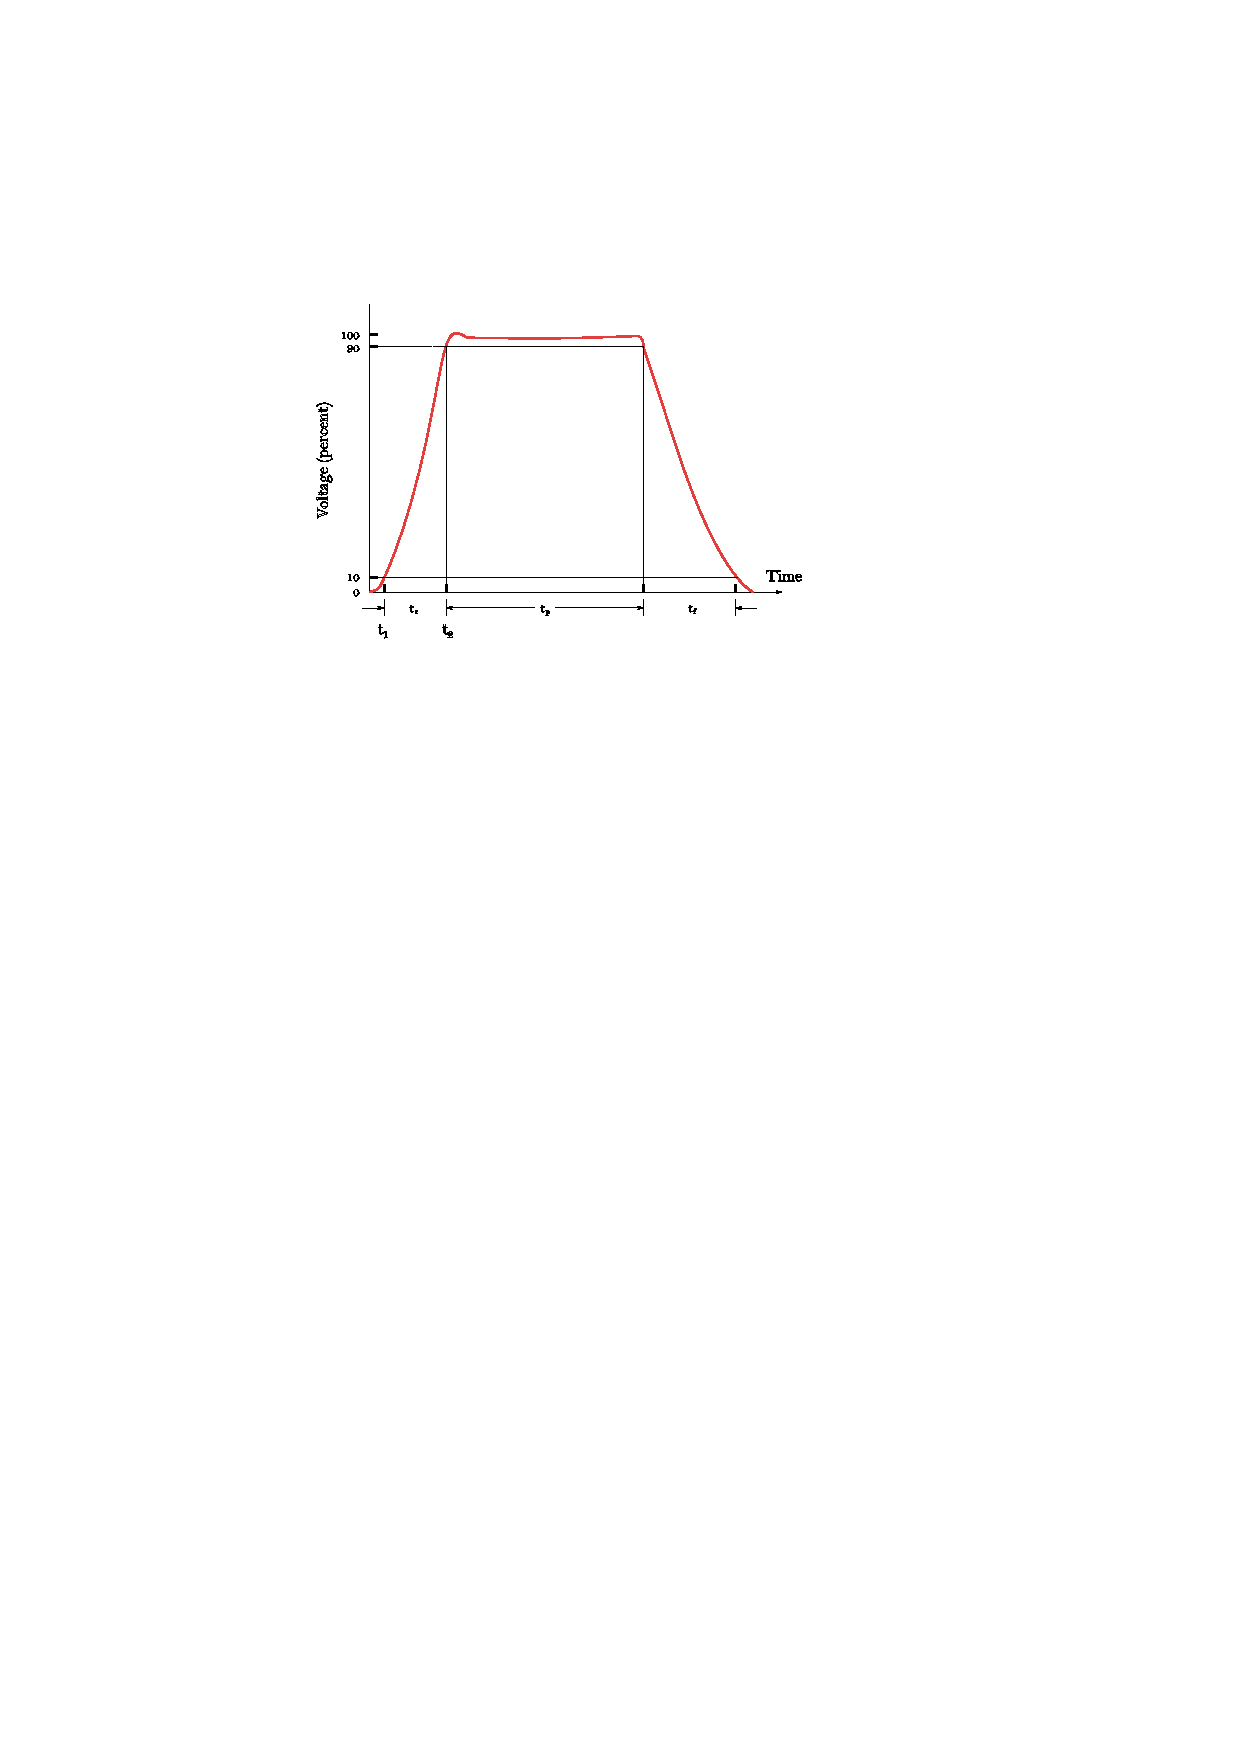
\includegraphics[clip, trim=5cm 18.5cm 7cm 5cm, width=0.7\textwidth]{graph1.pdf}
	\caption{Title}
	\label{fig:somthing}
\end{figure}

El tiempo de subida $t_r$ está dado por

\begin{align}
	t_r = t_1 - t_2
\end{align}

Donde $t_1$ es el tiempo en el cual el voltaje en el capacitor alcanza un valor de $0.1E$. Al sustituir la ecuación (2) en (1) obtenemos

\begin{align}
	0.1E &= E(1 - e^{-\frac{t_1}{RC}}) \nonumber \\
	0.1 &= 1 - e^{-\frac{t_1}{RC}} \nonumber \\
	0.9 &= e^{-\frac{t_1}{RC}} \nonumber \\
	e^{\frac{t_1}{RC}} &= \frac{10}{9} \nonumber \\
	\frac{t_1}{RC} &= \ln \left( \frac{10}{9} \right)
\end{align}

Es decir:

\begin{align}
	t_1 = RC \ln \left( \frac{10}{9} \right) \approx 0.1RC
\end{align}

De manera similar, el tiempo $t_2$ es el tiempo en el cual el voltaje en el capacitor alcanza un valor de $0.9E$, es decir:

\begin{align}
	0.9E &=  E(1 - e^{-\frac{t_2}{RC}}) \nonumber \\
	0.9 &=  1 - e^{-\frac{t_2}{RC}} \nonumber \\
	e^{\frac{t_2}{RC}} &= 10 \nonumber \\
	\frac{t_2}{RC} &= \ln (10) \nonumber \\
	t_2 &= RC \ln (10)
\end{align}

Es decir:

\begin{align}
	t_2 = RC \ln (10) = 2.3RC	
\end{align} 

Habiendo calculado los tiempos $t_1$ y $t_2$ podemos calcular fácilmente el tiempo de subida de la señal de la figura 1 como

\begin{align}
	t_r = t_2 - t_1 = 2.3RC - 0.1RC = 2.2RC
\end{align}

\section{Ejemplo}

Sea $R = \qty{10}{\kilo \ohm}$ y  $C = \qty{1}{\micro \farad}$

\begin{figure}[H]
	\centering
	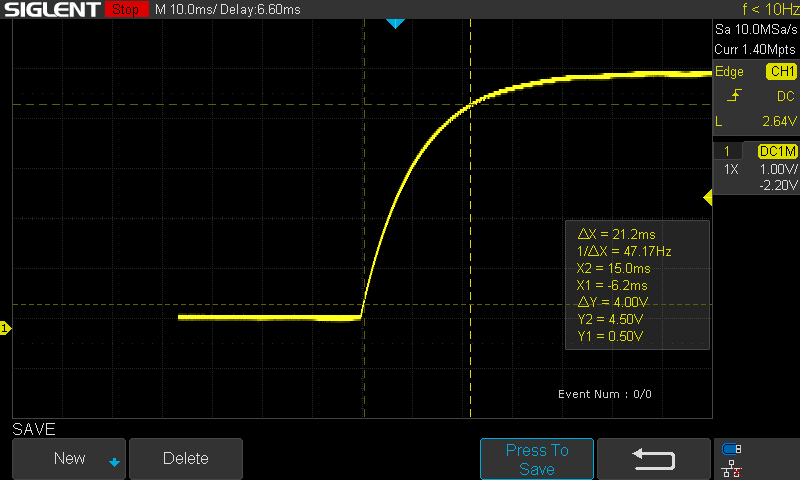
\includegraphics[width=1.0\textwidth]{SDS00001}
	\caption{Title}
	\label{fig:graph}
\end{figure}

\end{document}